\documentclass[11pt]{article}

\title{\color{navyblue} Differences-in-Differences with Spatial Spillover}
% \subtitle{Subtitle}
\author{\normalsize Kyle Butts\\{\footnotesize Univ. of Colorado, Boulder}}
\date{\footnotesize\today}

% Margins ----------------------------------------------------------------------

\usepackage[margin=1.25in]{geometry}

% AMS --------------------------------------------------------------------------

\usepackage{amsmath}
\usepackage{amsfonts}
\usepackage{amsthm}
\usepackage{graphicx}


% Line Spacing -----------------------------------------------------------------

\renewcommand{\baselinestretch}{1.5}


% Font -------------------------------------------------------------------------

\usepackage[T1]{fontenc}
\usepackage[default]{lato} % Lato as text font
% \usepackage[utopia, varg]{newtxmath}
% \renewcommand{\rmdefault}{futs} % Utopia as text font 

% Small adjustments to text kerning
\usepackage{microtype}

% Remove annoying over-full box warnings
\vfuzz2pt 
\hfuzz2pt


% Tikz support -----------------------------------------------------------------

\usepackage{tikz}


% Color Palette ----------------------------------------------------------------

\usepackage{xcolor}

% https://www.materialpalette.com/colors
\definecolor{dark-maroon}{HTML}{5D0F0D}
\definecolor{navyblue}{HTML}{0A3044}

% From Davidson Mackinnon
\definecolor{dm-blue}{HTML}{086fbd}
\definecolor{dm-red}{HTML}{ba3132}
\definecolor{dm-green}{HTML}{3f7e32}

% https://www.viget.com/articles/color-contrast/
\definecolor{purple}{HTML}{5601A4}
\definecolor{navy}{HTML}{0D3D56}
\definecolor{ruby}{HTML}{9a2515}
\definecolor{alice}{HTML}{107895}
\definecolor{daisy}{HTML}{EBC944}
\definecolor{coral}{HTML}{F26D21}
\definecolor{kelly}{HTML}{829356}
\definecolor{cranberry}{HTML}{E64173}
\definecolor{jet}{HTML}{131516}
\definecolor{asher}{HTML}{555F61}
\definecolor{slate}{HTML}{314F4F}


% Hyperlinks -------------------------------------------------------------------

\usepackage{hyperref}
\hypersetup{
    colorlinks= true,
    citecolor= dark-maroon,
    linkcolor= dark-maroon,
    filecolor= dark-maroon,      
    urlcolor= dark-maroon,
}


% Citations --------------------------------------------------------------------

% note, natbib provides better hyperlinking
\usepackage{natbib}
\bibliographystyle{econ-aea}


% Define Theorems --------------------------------------------------------------

% Put proper spacing after Theorem #. 
\newtheoremstyle{spacing}
{}%          Space above, empty = `usual value'
{}%          Space below
{}%  Body font
{}%          Indent amount (empty = no indent, \parindent = para indent)
{\bfseries\color{navyblue}}% Thm head font
{.}%         Punctuation after thm head
{2.5mm}%  Space after thm head: \newline = linebreak
{}%          Thm head spec

% note, theorem is the name that goes in \begin{} and Theorem is the name displayed as Theorem 1
\theoremstyle{spacing}
\newtheorem{theorem}{Theorem}
\newtheorem{proposition}{Proposition}
\newtheorem{assumption}{Assumption}
\newtheorem{example}{Example}


% Custom Math Definitions ------------------------------------------------------

\newcommand{\expec}[1]{\mathbb{E}\left[#1\right]}%
\newcommand{\condexpec}[2]{\mathbb{E}\left[#1 \ \vert \ #2\right]}%
\newcommand{\prob}[1]{\mathbb{P}\left[#1\right]}%
\newcommand{\var}[1]{\mathrm{Var}\left[#1\right]}%
\newcommand{\cov}[1]{\mathrm{Cov}\left[#1\right]}%
\newcommand{\one}{\mathbf{1}}


% Titlepage --------------------------------------------------------------------

% \maketitle
\usepackage{titling}
\usepackage{setspace}

% title
\pretitle{\begin{spacing}{1}\begin{flushleft}\huge}
\posttitle{\end{flushleft}\end{spacing}\vspace{-5mm}}
% author, note don't use \and 
\preauthor{\begin{flushleft}\LARGE}
\postauthor{\end{flushleft}\vspace{-7.5mm}}
% date
\predate{\begin{flushleft}\Large\color{asher}}
\postdate{\end{flushleft}\vspace{-5mm}}

% Abstract
\renewenvironment{abstract}
 {\noindent\rule{\linewidth}{.5pt}\noindent}
 {\noindent\rule{\linewidth}{.5pt}}

% alternative abstract
% \renewenvironment{abstract}
% {
%   \centerline {\large \bfseries \scshape \color{navyblue} Abstract}
%   \begin{quote}
% }
% {\end{quote}}


% Section and Subsection Styling -----------------------------------------------

\usepackage[explicit]{titlesec}

\titleformat{\section}
  {\Large \bf \color{navyblue}}
  {\thesection \,---}
  {0.25em}
  {#1}
  
\titleformat{\subsection}
  {\fontsize{11}{10}\it}
  {\thesubsection.}
  {1em}
  {#1}

% Don't number subsubsection
\setcounter{secnumdepth}{2}

% Footnote ---------------------------------------------------------------------

% Spacing between footnotes on same page
\addtolength{\footnotesep}{1mm}

% Space after footnote number
\let\oldfootnote\footnote
\renewcommand\footnote[1]{\oldfootnote{\ #1}}

% No footnote line
\renewcommand\footnoterule{}

% No supsercript in footer
\makeatletter
\renewcommand\@makefntext[1]{%
    \parindent 1em \noindent
    \hb@xt@1.8em{\hss\normalfont\@thefnmark.\hfill}#1
  }
\makeatother




% Enumerate/Itemize ------------------------------------------------------------

\usepackage{enumitem}
\setitemize{labelindent=0.5em,labelsep=0.25cm,leftmargin=*}
\setenumerate{labelindent=0.5em,labelsep=0.25cm,leftmargin=*}


% Table and Figure labelling ---------------------------------------------------

\usepackage{caption}

\DeclareCaptionLabelSeparator{threedash}{\,---\,}
\DeclareCaptionFont{navyblue}{\color{navyblue}}
\DeclareCaptionFont{jet}{\color{jet}}
\captionsetup[table]{format=plain, labelsep=threedash, font={navyblue, bf}}
\captionsetup[figure]{format=plain, labelsep=threedash, font={navyblue, bf}}

% Alternative: Left align captions
% \captionsetup[table]{labelfont=it, textfont={navyblue, bf}, labelsep=newline, justification=raggedright, singlelinecheck=off}
% \captionsetup[figure]{labelfont=it, textfont={navyblue, bf}, labelsep=newline, justification=raggedright, singlelinecheck=off}

% multifigure with \caption
% \begin{subfigure}\caption{} \end{subfigure}
\usepackage{subcaption}
\captionsetup[subfigure]{format=plain, font={jet, footnotesize, bf}}


% Tables -----------------------------------------------------------------------

% Fix \input with tables
% \input fails when \\ is at end of external .tex file

\makeatletter
\let\input\@@input
\makeatother

% Make tables/figures wider than \textwidth using:
% \begin{adjustbox}{width = 1.2\textwidth, center}
% \end{adjustbox}
\usepackage{adjustbox}

% Slighty more spacing between rows
\usepackage{array}
\renewcommand\arraystretch{1.2}

% Table with easy to use footnotes
% \begin{threeparttable}
%    \begin{tabular} ... \end{tabular}
%    \begin{tablenotes}
%        \item \textit{Notes.}
%    \end{tablenotes}  
% \end{threeparttable}
\usepackage[flushleft]{threeparttable}
\setlength\labelsep{0pt}

% \toprule, \cmidrule, \bottomrule
\usepackage{booktabs}

% If tables are too narrow, fill columns using:
% \begin{tabularx}{\linewidth}{cols}
% col-types: X - center, L - left, R -right
% If you want relative scale for columns: 
% >{\hsize=.8\hsize}X/L/R
\usepackage{tabularx}
\newcolumntype{L}{>{\raggedright\arraybackslash}X}
\newcolumntype{R}{>{\raggedleft\arraybackslash}X}
\newcolumntype{C}{>{\centering\arraybackslash}X}

% Shorter multicolumn commands
\newcommand{\mcc}[1]{\multicolumn{1}{c@{}}{#1}}
\newcommand{\mcl}[1]{\multicolumn{1}{l@{}}{#1}}
\newcommand{\mcr}[1]{\multicolumn{1}{r@{}}{#1}}

% d column
\usepackage{dcolumn}
\newcolumntype{d}[1]{D..{#1}}

% Landscape table 
% \begin{landscape} \pagestyle{lscaped} table... \end{landscsape}
% \usepackage{pdflscape} - rotates page left-side up in pdf
% \usepackage{lscape} - does not rotate page, only figure/table

\usepackage{pdflscape}

% For landscape, fix page number location
\usepackage{fancyhdr}
\fancypagestyle{lscaped}{%
    \fancyhf{}
    \renewcommand{\headrulewidth}{0pt}
    \textnormal
    \fancyfoot{%
        \tikz[remember picture,overlay]
        \node[outer sep=2.5cm,above,rotate=90] at (current page.east) {\thepage};
    }
}
  

% ------------------------------------------------------------------------------

\addbibresource{references.bib}

\begin{document}

% ------------------------------------------------------------------------------
\begin{titlepage}
    \maketitle
    
    \begin{abstract}
        Empirical work often uses treatment variables defined by geographic boundaries. When researchers ignore the common problem that the effects of treatment cross over borders, classical difference-in-differences estimation produces biased estimates for the average treatment effect. In this paper, I decompose this bias in two parts. First, the control group no longer identifies the counterfactual trend because their outcomes are affected by treatment. Second, changes in treated units' outcomes reflect the effect of their own treatment status and the effect from the treatment status of ``close'' units. I use Monte Carlo simulations to demonstrate when the biases are particularly large. Further, I show that a common solution used in the literature of removing `contaminated' control units only prevents the first source of bias. Lastly, I propose improved estimation strategies that can remove both sources of bias. I highlight the importance of considering spillovers by revisiting analysis of the Tennessee Valley Authority.
    \end{abstract}
\end{titlepage}
% ------------------------------------------------------------------------------

% ------------------------------------------------------------------------------
\section{Introduction}
% ------------------------------------------------------------------------------

Empirical work in economics often considers treatment assigned by geographic boundaries such as cities, counties, and states. Potentially, the effect of these treatments do not stay within these boundaries whether it be from people crossing borders to access treatment (imperfect compliance) or from general equilibrium effects influencing neighboring areas. Despite the problem of spatial spillovers being common across many settings, \citet{Berg_Streitz_2019} document that little empirical analysis takes the problem seriously. In a survey of eight top economics and finance journals in 2017, they find that only 21 articles out of 108 that run difference-in-differences estimation discuss spillovers.\footnote{The articles surveyed are American Economic Review, Econometrica, the Journal of Political Economy, the Quarterly Journal of Economics, the Review of Economic Studies, the Journal of Finance, the Journal of Financial Economics, and the Review of Financial Studies.} In this paper, I show that failing to account for spatial spillovers can lead to poorly identified estimates of treatment effects.

In the causal inference literature, researchers assume that a unit's potential outcome does not depend on the treatment status of any other unit -- what \citet{Rubin_1980} calls the Stable Unit Treatment Value Assumption (SUTVA). This article considers a common violation of SUTVA in a process I label `spatial spillovers' where the treatment assignment of `close' units' affects outcomes of nearby units.\footnote{Close can refer to many different things, e.g. geographic distance, economic distance such as supply chains, node distance in a graph, or social relationships in schools or cities.} Typically researchers are interested in the `direct effect' on the treated units.\footnote{This is sometimes called the `partial equilibrium' effect or the `local effect'.} In the presence of spatial spillovers, I show using a potential outcomes framework that the difference-in-differences estimate identifies the direct effect of treatment (the estimand of interest) plus two additional bias terms resulting from the spillovers.

The intuition for the two bias terms resulting from spillovers is as follows. First, untreated units that are `close' to treated units experience effects of treatment and therefore these `control' units fail to identify the counterfactual trend. When estimating by difference-in-differences, the spillover onto the `close' control units is averaged into the untreated units' change in outcomes. In this case, the spillover is subtracted from the estimated treatment effect and biases the estimate in the opposite sign of the spillover effect. For example, consider a factory opening in a county. Agglomeration economies suggest that neighboring counties would also benefit from knowledge spillovers and improved access to supply chain \citep{Duranton_Puga_2003}. The treatment effect estimate is negatively biased because the change in outcome in neighboring counties is higher than it would be absent treatment. Researchers would therefore underestimate the positive benefits of treatment.\footnote{If the policy maker had a welfare function that included both treated and neighboring counties, they would fail to count the positive benefits of the control units and they would underestimate the positive benefits on the treated units. Difference-in-differences estimation would therefore result in double undercounting.}

Second, changes in treated units' outcomes reflect the effect of their own treatment status and the effect from the treatment status of ``close'' units. The spillover onto other treated units is averaged into the treated units' change in outcomes. Therefore the bias of treatment effect is the same sign as the sign of the spillover. Continuing with our example, two factory openings in neighboring counties might cause the benefit of each individual factory to increase due to agglomeration forces. The estimated treatment effect will count the `direct` effect of the factory opening as well as the benefit of the agglomeration economies. Therefore the treatment effect will be positively biased due to the positive spillover onto also treated units. 

These biases can be written as functions of the potential outcomes in my framework and can be used by researchers to sign or bound the bias using insight from their economic context. The magnitude of the bias depends on two factors: the size of the spillovers and the number of units affected by spillovers. If spillovers are quite large in magnitude or spread far over distance, then the bias will generally be large. Th results of this paper enable researchers to estimate bounds for it by making assumptions about the average size of the spillover effect and the number of units affected. I use Monte Carlo simulations to quantify the magnitude of bias in various spillover settings.

In the survey by \citet{Berg_Streitz_2019}, only eight of the 21 papers that discuss spillovers control for this potential source of bias in their primary empirical specification to prevent bias in the estimation of treatment effects. The other thirteen papers usually first estimate the direct effect without controlling for spillovers and then seperately estimate the spillover effects. This paper shows that not controlling for spillovers produces biased estimates of the direct effect. 

Of the eight papers that include spillovers directly in their estimation strategy, six simply drop the control units they suspect to be affected by spillovers. Since this is a common strategy used by researchers, I use Monte Carlo simulations to show that this method is effective in the case where spillovers \textit{only} occur onto control units. In the presence of spillover onto also treated units, the estimates for the direct effect will still be biased. Dropping control unit observations, however, makes estimates less precise, so parameterizing the spillover function may be a better strategy especially in the case where a high proportion of control units would need to be removed.

Removing both sources of bias requires a researcher to take a stance and parameterize a functional form for the spillovers. The particular functional form depends on the context of the application. However, there are a few practical considerations. First, the researcher should argue whether spillovers on control units and on treated units exist. Second, they should argue what the maximum distance these spillovers can occur. Last, they should consider if spillovers are additive in the number of nearby units that are treated. 

In section \ref{sec:monte_carlo}, I use Monte-Carlo simulations to emphasize when misspecificied spillovers still remove most of the bias and when they fail to do so. 

% @TODO: Discuss effectiveness under misspecification of spillovers (correct distance and additive/non-additive).

% ------------------------------------------------------------------------------
\subsection{Contribution}
% ------------------------------------------------------------------------------

The literature considering spillovers primarily has focused on ``within-group'' spillovers where units are in distinct groups and outcomes depend on the treatment status within the observation's group only.\footnote{For example, researchers consider peer effects within schools. In this case, each school constitutes a group and it is assumed that outcomes do not depend on other schools' treatment status, i.e. SUTVA is satisfied between-groups. Estimation of spillover effects in this case is done in a `partial intereference' framework that compares ``control'' units in a partially treated group with control units in completely untreated groups. \citet{Angelucci_DiMaro_2016} provides a summary for estimation of spillover effects in within-group settings. Examples in the literature include: \citet{Halloran_Struchiner_1995} consider community-vaccine rates in epidemology; \citet{Miguel_Kremer_2004} consider deworming programs in Kenyan schools; \citet{Sobel_2006} considers interference in the Moving to Opportunity Program; and \citet{Angrist_2014} studies the context of school peer effects.} However, spatial settings such as counties do not feature distinct groups which allow for the researcher to separate areas into distinct non-overlapping groups (a county is connected to all other counties by some chain of neighbors). My paper considers a more general form of interference. Identification in this framework requires the researcher to either identify control units that are free from spillovers (far-away from treatment) or to parameterize how control units are affected by treatment.

\citet{Vazquez-Bare_2019} models within-group spillovers such that their exposure mapping is only a function of unit $i$'s group's treatment vector. He develops a potential outcomes framework which assumes that potential outcomes are a function of both own treatment-status $D_i$ and a function of the vector of treatment assignments $h(\vec{D}, i)$. The function $h(\vec{D}, i)$ is referred to as an exposure mapping and adding this to the potential outcomes framework allows me to explicitly model SUTVA violations. Using this framework, \citet{Vazquez-Bare_2019} shows that a difference in means comparison between treated and control units is a biased estimated for the treatment effect. 

My paper uses this potential outcome framework in the case where treatment spillover is not limited to within-group spillovers and considers estimation of treatment effects by difference-in-differences. 

\citet{Sävje_Aronow_Hudgens_2019} consider a similar potential outcome framework as \citet{Vazquez-Bare_2019}, but they instead include spillovers as a part of their definition of ``treatment effect''. That is, a treated unit's treatment effect is defined as the direct effect \textit{and} the general equilibrium spillover effects. Then, the authors describe how the average treatment effect (ATE) estimated by difference-in-differences averages over both individual heterogeneity and, central to their contribution, over heterogeneity in the exposure mapping, $h(\vec{D}, i)$. My paper develops a strategy to allow researchers to seperately identify treatment effects and spillovers.\footnote{These estimates can be combined afterwards to estimate their definition of average treatment effect. The further advantage is that `net' treatment effects can be estimated at different levels of exposure which is more relevant for future policy decisions.}

There are a few papers that discuss estimation of treatment effects with spatial spillovers using the difference-in-differences framework. \citet{Clarke_2017} finds an explicit form for bias when estimating a difference-in-differences model. However, their model only allows spillovers onto control units and assumes spillovers are constant regardless on the number of nearby treated units. \citet{Berg_Streitz_2019} and \citet{Verbitsky-Savitz_Raudenbush_2012} identifies biases in estimation of the direct effect for a specific potential outcome function where $h(\vec{D}, i)$ is the proportion of treated contiguous counties. Finally, \citet{Delgado_Florax_2015} consider the case where the exposure mapping is defined by a spatial weights matrix $W\vec{D}$ that enters linearly into the potential outcomes. This does not allow for the coefficient to change for control and treated units.\footnote{Although, one could change the weighting matrix to make ad-hoc assumption of the signs and relative magnitudes of spillovers onto treated and control units, but this allows for less data-driven estimation.}

My paper derives an explicit form for this bias in terms of general potential outcomes which allows my results to capture many different forms of spillovers. For the above papers, if I assume the particular functional forms for potential outcomes, I arrive at the same bias equation as theirs if they have one derived explicitly. My paper also advances the literature by considering estimation of direct effects and spillover effects in event-study framework which allows for the common occurence of staggered treatment adoption.

Lastly, I contribute to a literature in urban economics on local place-based policies. Using structural urban models, \citet{Kline_Moretti_2014b} show that the `local' or partial equilibrium effects of a place-based policy are offset in part by indirect or general equilibrium effects. I contribute to estimating aggregate effects of place-based policies by showing that typical estimation strategies can underestimate the local effect by ignoring spillovers. As an example, I revisit the analysis of the Tennessee Valley Authority by \citet{Kline_Moretti_2014}. The Tennessee Valley Authority was a large push to bring electrification to the Tennessee Valley with the goal of improving the manufacturing sector there. The scale of the program was large and the pro-manufacturing benefits likely spread further than the Authority's boundary due to the electrification infrastucture and agglomeration economies. I show that estimation by difference-in-differences fails to account for these spillovers and for different outcome variable it underestimates and overestimates the local effect, depending on the sign of the spillovers. 

The rest of the paper is structured as follows. Section \ref{sec:po_framework} presents the potential outcomes framework, defines the estimand of interest, and shows the resulting bias from estimating a classical difference-in-differences model. Section \ref{sec:monte_carlo} presents Monte Carlo simulations to illlustrate the bias result and to evaluate currently used solutions in the literature. Section \ref{sec:tva} presents an application for evaluating the Tennessee Valley Authority program. Section \ref{sec:event_study} discusses briefly how to incorporate spillovers into event-study estimation following the insights from \citet{Callaway_Sant’Anna_2020}.



% ------------------------------------------------------------------------------
\section{Potential Outcomes Framework}
\label{sec:po_framework}
% ------------------------------------------------------------------------------

Following the canonical difference-in-difference framework, there is a time $t_0$ where treatment turns on and remains on afterwards. This framework can be extended in section \ref{sec:event_study}. As in \citet{Vazquez-Bare_2019}, potential outcomes for unit $i$ at time $t$ are a function of own treatment-status $D_i$ and, departing from the standard potential outcomes framework, of a function of the entire vector of treatment assignments $h(\vec{D}, i)$ where $\vec{D} \in \{0,1 \}^n$ denotes the $n$-dimensional vector of all unit treatments. The potential outcomes are denoted $Y_{i,t}(D_i, h(\vec{D}, i)$). The function $h(\vec{D}, i)$ is referred to as an `exposure mapping' and is a non-negative scalar- or vector- valued function. The exposure mapping measures the intensity at which unit $i$ is affected by spatial spillovers. When unit $i$ is sufficiently `far' away, it has no exposure to spatial spillovers and $h(\vec{D}, i) = 0$. The exposure mapping formalizes the SUTVA violation in that potential outcomes are affected by other unit's treatment assignment as summarized by $h(\vec{D}, i)$. To help better understand the exposure mapping function, I give three examples of $h(\vec{D}, i)$ that are commonly used in the literature.

First, $h(\vec{D}, i)$ can be a 0/1 variable that equals one only if there is a treated unit within $\bar{d}$-miles of unit $i$.\footnote{Similarly a dummy for counties that share borders is commonly used.} Let $d(i,j)$ be a geographic distance measure which tells the distance unit $i$ is from unit $j$.  In this case \begin{equation}\label{eq:h_within}
    h(\vec{D}, i) = \max_{i \neq j} D_j * 1[ d(i,j) < \bar{d} ] 
\end{equation}
This exposure mapping is useful when it is assumed that spillovers do not decay over distance until $\bar{d}$ and the number of neighboring units treated do not impact the intensity of spillovers. For example, this exposure mapping likely applies in the context of new library creation \citep{Berkes_Nencka_2020}. In this case the distance $\bar{d}$ would be the maximum distance people would travel to a nearby library. Access to a neighboring town library is binary in nature, so it does not matter whether you can access 1 or more nearby libraries, so the binary exposure mapping is a good approximation to spillovers in this context.  

Second, $h(\vec{D}, i)$ can be a function that equals the proportion of the k-nearest neighbors that are treated, i.e. \begin{equation}\label{eq:h_within}
    h(\vec{D}, i) = 1/k \sum_{j \in K(i)} D_j,
\end{equation}
where $K(i)$ is the index of unit $i$'s k-nearest neighbors. This exposure mapping is no longer binary, so the intensity of spillovers depend on the number of units treated. In the context of large store openings, this exposure mapping captures the additive nature of agglomeration economies. As more nearby counties receive new stores, the agglomeration forces increase \citep{Basker_2005}.

Last, is the spatial decay function where exposure decreases with distance. In this case, spillover intensity is the sum across all treated observations' decay term, i.e. \begin{equation}\label{eq:h_decay}
    h(\vec{D}, i) = \sum_{j \neq i} D_j e^{-\alpha d(i,j)}.
\end{equation} 
This exposure mapping allows for the intensity of spillovers to depend on distance to treatment and also is additive in the number of nearby units treated.\footnote{However, this specification assumes that all units are affected by all other units. This creates problems with inference because it implies potential correlation between all units' error terms. For this reason, this function often is summed over only the $k$-nearest neighbors or over units within $\bar{d}$ miles.} The speed of spillover decay over distance depends on the parameter $\alpha$ that can be calibrated by the researcher or estimated using non-linear least squares. In the literature on R\&D investment, \citet{Keller_2002} uses a modified version of this exposure mapping where $D_j$ is country $j$'s R\&D expenditure. 

After chosing an exposure mapping that makes sense in the economic context, a researcher must also specify the functional form of the potential outcomes. Typically, the spillover function enters into the regression linearly and potentially the coefficient is allowed to differ by treatment status. 



% ------------------------------------------------------------------------------
\subsection{Spatial Spillovers}
% ------------------------------------------------------------------------------

With the potential outcomes defined, I now formalize what is meant by `spatial spillovers'. I define `spillover onto control units' as: \[
    Y_{it}(0, h(\vec{D}, i)) - Y_{it}(0, 0).
\] 
The spillover measures the difference in non-treated potential outcomes between being exposed at intensity $h(\vec{D}, i)$ and not being exposed. Then, the average spillover effect onto control units averages over potential heterogeneity in spillovers and over heterogeneity in exposure intensity $h(\vec{D}, i)$: \[
    \tau_{\text{spill,control}} \equiv \mathbb{E} \left[ Y_{it}(0, h(\vec{D}, i)) - Y_{it}(0, 0) \ \vert \ D_i = 0 \right].
\]

To emphasize, the average spillover effect onto conrol units averages over each control unit's exposure mapping. For example, assume the potential outcomes is additively linear in $D_i$ and $h(\vec{D}, i)$ and that the coefficient $\beta_{\text{spill,control}}$ measures the effect of $h(\vec{D}, i)$ on outcome $Y$ among control units. Then an individual control unit's spillover effect is $\beta_{\text{spill,control}} \ h(\vec{D}, i)$. The average spillover effect onto control unit would therefore be $\tau_{\text{spill,control}} = \beta_{\text{spill,control}} * \mathbb{E} \left[ h(\vec{D}, i)\right]$, i.e. the average over all control units exposure mapping.

Similarly, we define the average spillover effect onto also treated units as: \[ 
    \tau_{\text{spill,treated}} \equiv \mathbb{E} \left[ Y_{it}(1, h(\vec{D}, i)) - Y_{it}(1, 0) \ \vert \ D_i = 1 \right].
\] 

It is important to clarify what I am assuming is the estimand of interest researchers would like to estimate when using difference-in-differences. I assume that what the `average treatment effect' is trying to measure in this context is what I will call the `direct effect of treatment': \[
    \tau_{\text{direct}} = \mathbb{E} \left[ Y_{it}(1, 0) - Y_{it}(0, 0) \ \vert \ D_i = 1 \right],
\] 
which measures the effect of being treated in the absence of exposure to spillovers. This effect does not include the general equilibrium effects of multiple treated areas near one-another.

My definition of the direct effect of treatment differs from \citet{Sävje_Aronow_Hudgens_2019} where they define the average treatment effect as \[ 
    \mathbb{E} \left[ Y_{it}(1, h(\vec{D}, i)) - Y_{it}(0, h(\vec{D}, i)) \ \vert \ D_i = 1 \right],
\] 
where the expectation is over individuals and their exposures. I prefer the former because it allows for seperate identification of the direct effect of treatment and the spillover effects themselves. For example, a county deciding whether to implement a policy will want to consider the treatment effect plus the spillover at their current level of exposure. The estimand proposed by \citet{Sävje_Aronow_Hudgens_2019} returns the average of spillovers across levels of exposure and can not be used to predict spillovers at different levels.\footnote{Estimation of the direct effect and spillover effect can be combined to estimate the ATE as defined by \citet{Sävje_Aronow_Hudgens_2019}.}


% ------------------------------------------------------------------------------
\subsection{Bias in Difference-in-Differences Estimation}
% ------------------------------------------------------------------------------

In this section, I identify the two sources of bias in difference-in-differences estimation of the direct effect of treatment. For exposition, I will refer to one pre- and post-period, $t = 0$ and $t = 1$, but this can be replaced by averages across $Y$ in the pre-period and the post-period respectively. To estimate the `direct effect of treatment', researchers estimate the canonical two-way fixed effects model, 
\begin{equation}\label{eq:twfe}    
    y_{it} = \tau D_{it} + \mu_i + \mu_t + \epsilon_{it}.
\end{equation}

The estimator $\hat{\tau}$ is a biased estimate for $\tau_{\text{direct}}$ in the presence of spillovers. To show this, I first present the equivalent to the parallel counterfactual trends assumption in the context of the new potential outcome framework. 

\begin{assumption}[Parallel Counterfactual Trends]\label{eq:parallel}
    \[ 
        \mathbb{E}\left[ Y_{i1}(0, 0) - Y_{i0}(0, 0) \ \vert \ D_i = 1 \right] = 
        \mathbb{E}\left[ Y_{i1}(0, 0) - Y_{i0}(0, 0) \ \vert \ D_i = 0 \right]
    \]
\end{assumption}
This assumption states that in the absence of treatment and with zero exposure (not just the absence of individual $i$'s treatment), the change in potential outcomes from period 0 to 1 would not depend on treatment status. This generalizes to the classic parallel counterfactual trends when SUTVA is satisfied because then every unit has zero exposure.

Given that Assumption (\ref{eq:parallel}) holds, the estimate $\hat{\tau}$ from (\ref{eq:twfe}) can be decomposed as the direct effect and the two sources of spillover bias. The proof is given in Appendix \ref{sec:proofs}.

\begin{theorem}[Bias from Difference-in-Differences Estimation]\label{thm:bias}\ \\    
    If Assumption (\ref{eq:parallel}) holds, the expectation of the estimate $\hat{\tau}$ from (\ref{eq:twfe}) is
    \begin{align*}
        \mathbb{E}[\hat{\tau}] &= \underbrace{\mathbb{E}\left[ Y_{i1} - Y_{i0} \ \vert \ D_i = 1 \right] - \mathbb{E}\left[ Y_{i1} - Y_{i0} \ \vert \ D_i = 0 \right]}_{\text{Difference-in-Differences}} \\ 
        &= 
        \mathbb{E} \left[ Y_{i1}(1, \vec{0}) - Y_{i1}(0, \vec{0}) \mid D_i = 1 \right] + \mathbb{E} \left[ Y_{i1}(1, h(\vec{D}, i)) - Y_{i1}(1, \vec{0}) \mid D_i = 1 \right] \\
        &\quad - \mathbb{E} \left[ Y_{i1}(0, h(\vec{D}, i)) - Y_{i1}(0, \vec{0}) \mid D_i = 0 \right] \\
        &= \tau_{\text{direct}} + \tau_{\text{spill,treated}} - \tau_{\text{spill,control}}
    \end{align*}
\end{theorem}

The intuition behind the biases are as follows. First, the change in outcomes among treated units combines the direct effect and the spillover from nearby treated units. Therefore the first difference adds the average spillover effect onto the treated units, $\tau_{\text{spill,treated}}$. Second, the change in outcomes among control units combines the parallel counterfactual trend with the average spillover effect onto control units. Since $\hat{\tau}$ is found by subtracting this second difference, we subtract the average spillover effect onto the control, $\tau_{\text{spill,control}}$. 

Readers that are judging estimates in the presence of spillovers can use the following heuristics to sign the bias. If they suspect spillovers onto control units, the bias is the opposite sign of the spillover. If they suspect spillovers onto treated units, the bias is in the same sign of the spillover. The overall bias is the sum of the two.



% ------------------------------------------------------------------------------
\subsection{Bounding the Bias}
% ------------------------------------------------------------------------------

The previous section finds an explicit form of the bias when estimating (\ref{eq:twfe}). The explicit form of bias can be used by researchers to provide bounds on the bias in a manner simmilar to \citet{Rambachan_Roth_2020}. To provide bounds on the bias, researchers must identify the set $\Delta = [\underline{\Delta}, \overline{\Delta}]$ such that it contains the bias \[ 
    \tau_{\text{spill,treated}} - \tau_{\text{spill, control}} \in \Delta
\]

Choosing this set requires considerations of the economic context. It is guided by choices of parameterization of the exposure mapping and potential outcomes. To exemplify this bias, I will illustrate how a researcher would bound the bias in a simple example. I will consider the example of the effect of new libraries on school outcomes. Following the motivation above, I assume that spillovers occur for any county that is within $\bar{d}$ miles of a treated county, i.e. 
\begin{align}
    \label{eq:example_exposure}
    h(\vec{D}, i) \equiv \text{Near}_{it} = \max_{i \neq j} D_j * 1[ d(i,j) < \bar{d} ].
\end{align}
This specification is a simple one in that the spillover is not additive in the number of nearby treated counties and does not decay over distance before reaching $\bar{d}$. Since treated counties have access to their own library, I will assume that no spillovers on to treated units exist. The potential outcome is assumed to be additive in both treatment and in the exposure mapping:
\begin{align}
    \label{eq:example_po}
    \begin{split}
        y_{it} &= \beta_{\text{direct}} D_{it} + \beta_{\text{spill,control}} (1-D_{it}) \text{Near}_{it} + \mu_t + \mu_i + \varepsilon_{it},
    \end{split}
\end{align}
where $\mu_t$ and $\mu_i$ are unit and time fixed effects respectively. In this case, the spillover on an individual control unit is given by $\tau_{\text{spill,control}}$. 

If a researcher estimates (\ref{eq:twfe}), then the bias will be \[ 
    - \tau_{\text{spill,control}} = - \beta_{\text{spill,control}} \frac{\sum_{i: D_{it} = 0} \text{Near}_{it}}{N_C},
\] 
where $N_C$ are the number of control units respectively. Simply put, the bias will be negative one times the proportion of control units that receive spillover effects time the size of the effect on control units. Then the bound can be created by bounding $\beta_{\text{spill,control}}$ and the proportion of control units that receive spillovers.

With a chosen $\Delta$, the partially identified set is given by $[\hat{\tau} + \underline{\Delta}, \hat{\tau} + \overline{\Delta}]$. Inference on this set can be done using Fixed-Length Confidence Intervals as in \citet{Rambachan_Roth_2020}. The confidence interval can be formed using standard normal critical values and spatially adjusted standard errors following \citet{Conley_1999} since we are assuming a specific spatial relationship between outcomes: \[ 
    \left[ \hat{\tau} - \underline{\Delta} - z_{1 - \alpha/2} \text{SE}_{\hat{\tau}}, \ \hat{\tau} + \overline{\Delta} + z_{1 - \alpha/2} \text{SE}_{\hat{\tau}}\right].  
\]


% ------------------------------------------------------------------------------
\subsection{Improving Estimation by Parameterizing Spillovers}
% ------------------------------------------------------------------------------

The previous section shows how to estimate the magnitude of potential bias in the estimation of (\ref{eq:twfe}). However, parameterization of the potential outcomes and exposure mapping allows for unbiased estimates of $\tau_{\text{direct}}$ by controlling for the exposure mapping directly. This is recommended for two reasons. 

First, controlling for exposure mapping allows for unbiased estimates of the direct effect of treatmnet if the potential outcomes are correctly specified. In the case where potential outcomes are `somewhat' incorrectly specified, this can remove some of the bias in estimation. Simulations below highlight that since spillovers are likely to decay over distance, controlling for immediate neighbors removes a large portion of the average spillover effects.

Second, the spillover effects themselves are potentially relevant for policy makers. If treatment for a given area is positive and there are positive benefits to neighboring regions, the estimated benefits will double-understate the true effect of treatment. First, it will not include the neighboring units' benefit in the calculation. Second, since the treatment effect will subtract the neighboring units' benefit, the neighboring units' benefit will be \emph{double undercounted}. Similarly, a policy maker trying to determine the net benefits for a treated location must consider the direct effect and the spillover effect onto treated units. This is because the size of benefits created by the treatment depend on the number of treated units nearby.

There are a few practical considerations researchers should make when parametrizing the spillovers and the answers to the questions will depend ultimately on the economic context being studied. First, researchers should consider whether control units and/or treated units experience effects from the treatment status of other units. For example, in the context of library construction, treated units likely do not experience spillovers while close control units do. In the context of factory openings, both control and treated units likely experience spillovers. 

Second, a researcher must decide how far the spillovers can reasonably be experience and whether the effect decays over distance. Things such as driving distance or access via public transportation can be helpful in deciding which units are `close enough' to experience spillovers. There are two commonly used techniques to model treatment effect decay.\footnote{If the spillovers is due to crossing borders into the treated area, then a reasonable decision about whether the effect decays is the frequency in which people use the good. For example, libraries whose benefit is only experienced from frequent usage would suggest that the effect decays over distance. On the other hand, abortion clinics opening are used infrequently and therefore the effect likely doesn't decay over distance within a certain cutoff.} First, as seen above is to use an exponential decay function with regards to distance. The other option is to use a set of `cocentric donut' indicators which are easy to interpret. An example of this is shown in the empirical application in Section \ref{sec:tva}. 

Last, it is important for estimation to know if the spillovers are additive or non-additive in nature. If the number of nearby treated units matter, then the exposure mapping should sum over nearby treated units in some way. For example, in the context of library construction, the number of neighbors with libraries does not change the size of the spillover for it is access to \textit{any} library that matters. In the context of factory openings, though, agglomeration economies imply that the spillovers are additive in nature.




% ------------------------------------------------------------------------------
\section{Monte Carlo Simulations}
\label{sec:monte_carlo}
% ------------------------------------------------------------------------------

% ------------------------------------------------------------------------------
\subsection{Spillover on Controls Only}
% ------------------------------------------------------------------------------

I now turn to a series of Monte Carlo Simulations to highlight the importance for controlling for spillovers in simulations. I use the set of counties in the contiguous United States and the data generating process used is defined by the exposure mapping given in (\ref{eq:example_exposure}) with cutoff distance $\bar{d} = 40$ miles and the data generating process given in (\ref{eq:example_po}). A unit of observation is a US county and the periods are $t \in \{1, \dots, 20\}$ with treatment turning on after period $t = 10$. The intercepet is $\alpha = -2$, the fixed effects are generated by $\mu_t \sim N(0.2t, 0.1^2)$ and $\mu_i \sim N(6, 2^2)$, and the error term is $\varepsilon \sim N(0, 2^2)$. Last, the size of treatment and spillovers are as follows: $\beta_{\text{direct}} = 2$, $\beta_{\text{spill, control}} = 1$ and $\beta_{\text{spill, treat}} = 0$.

For the first simulation, I restrict spillovers only to occur among control units, i.e. $\beta_{\text{spill, treat}} = 0$, and estimate the two-way fixed effects model, (\ref{eq:twfe}). This data generating process where spillovers only occur onto control units matches what has been typically assumed in the literature. I assign treatment among counties randomly with various unconditional probabilities between 3 percent and 50 percent. The DGP is therefore 
\begin{equation}
    \label{eq:dgp1} 
    y_{it} = \mu_t + \mu_i + \beta_{\text{direct}} D_{it} + \beta_{\text{spill, control}} (1-D_{it}) \text{Near}_{it} + \varepsilon_{it}   
\end{equation}

\begin{figure}[tb!]
    \caption{Bias of $\hat{\tau}$ with Spillovers Effects \emph{only} on Control Units}
    \label{fig:bias_as_treat_prob}
    {\centering
        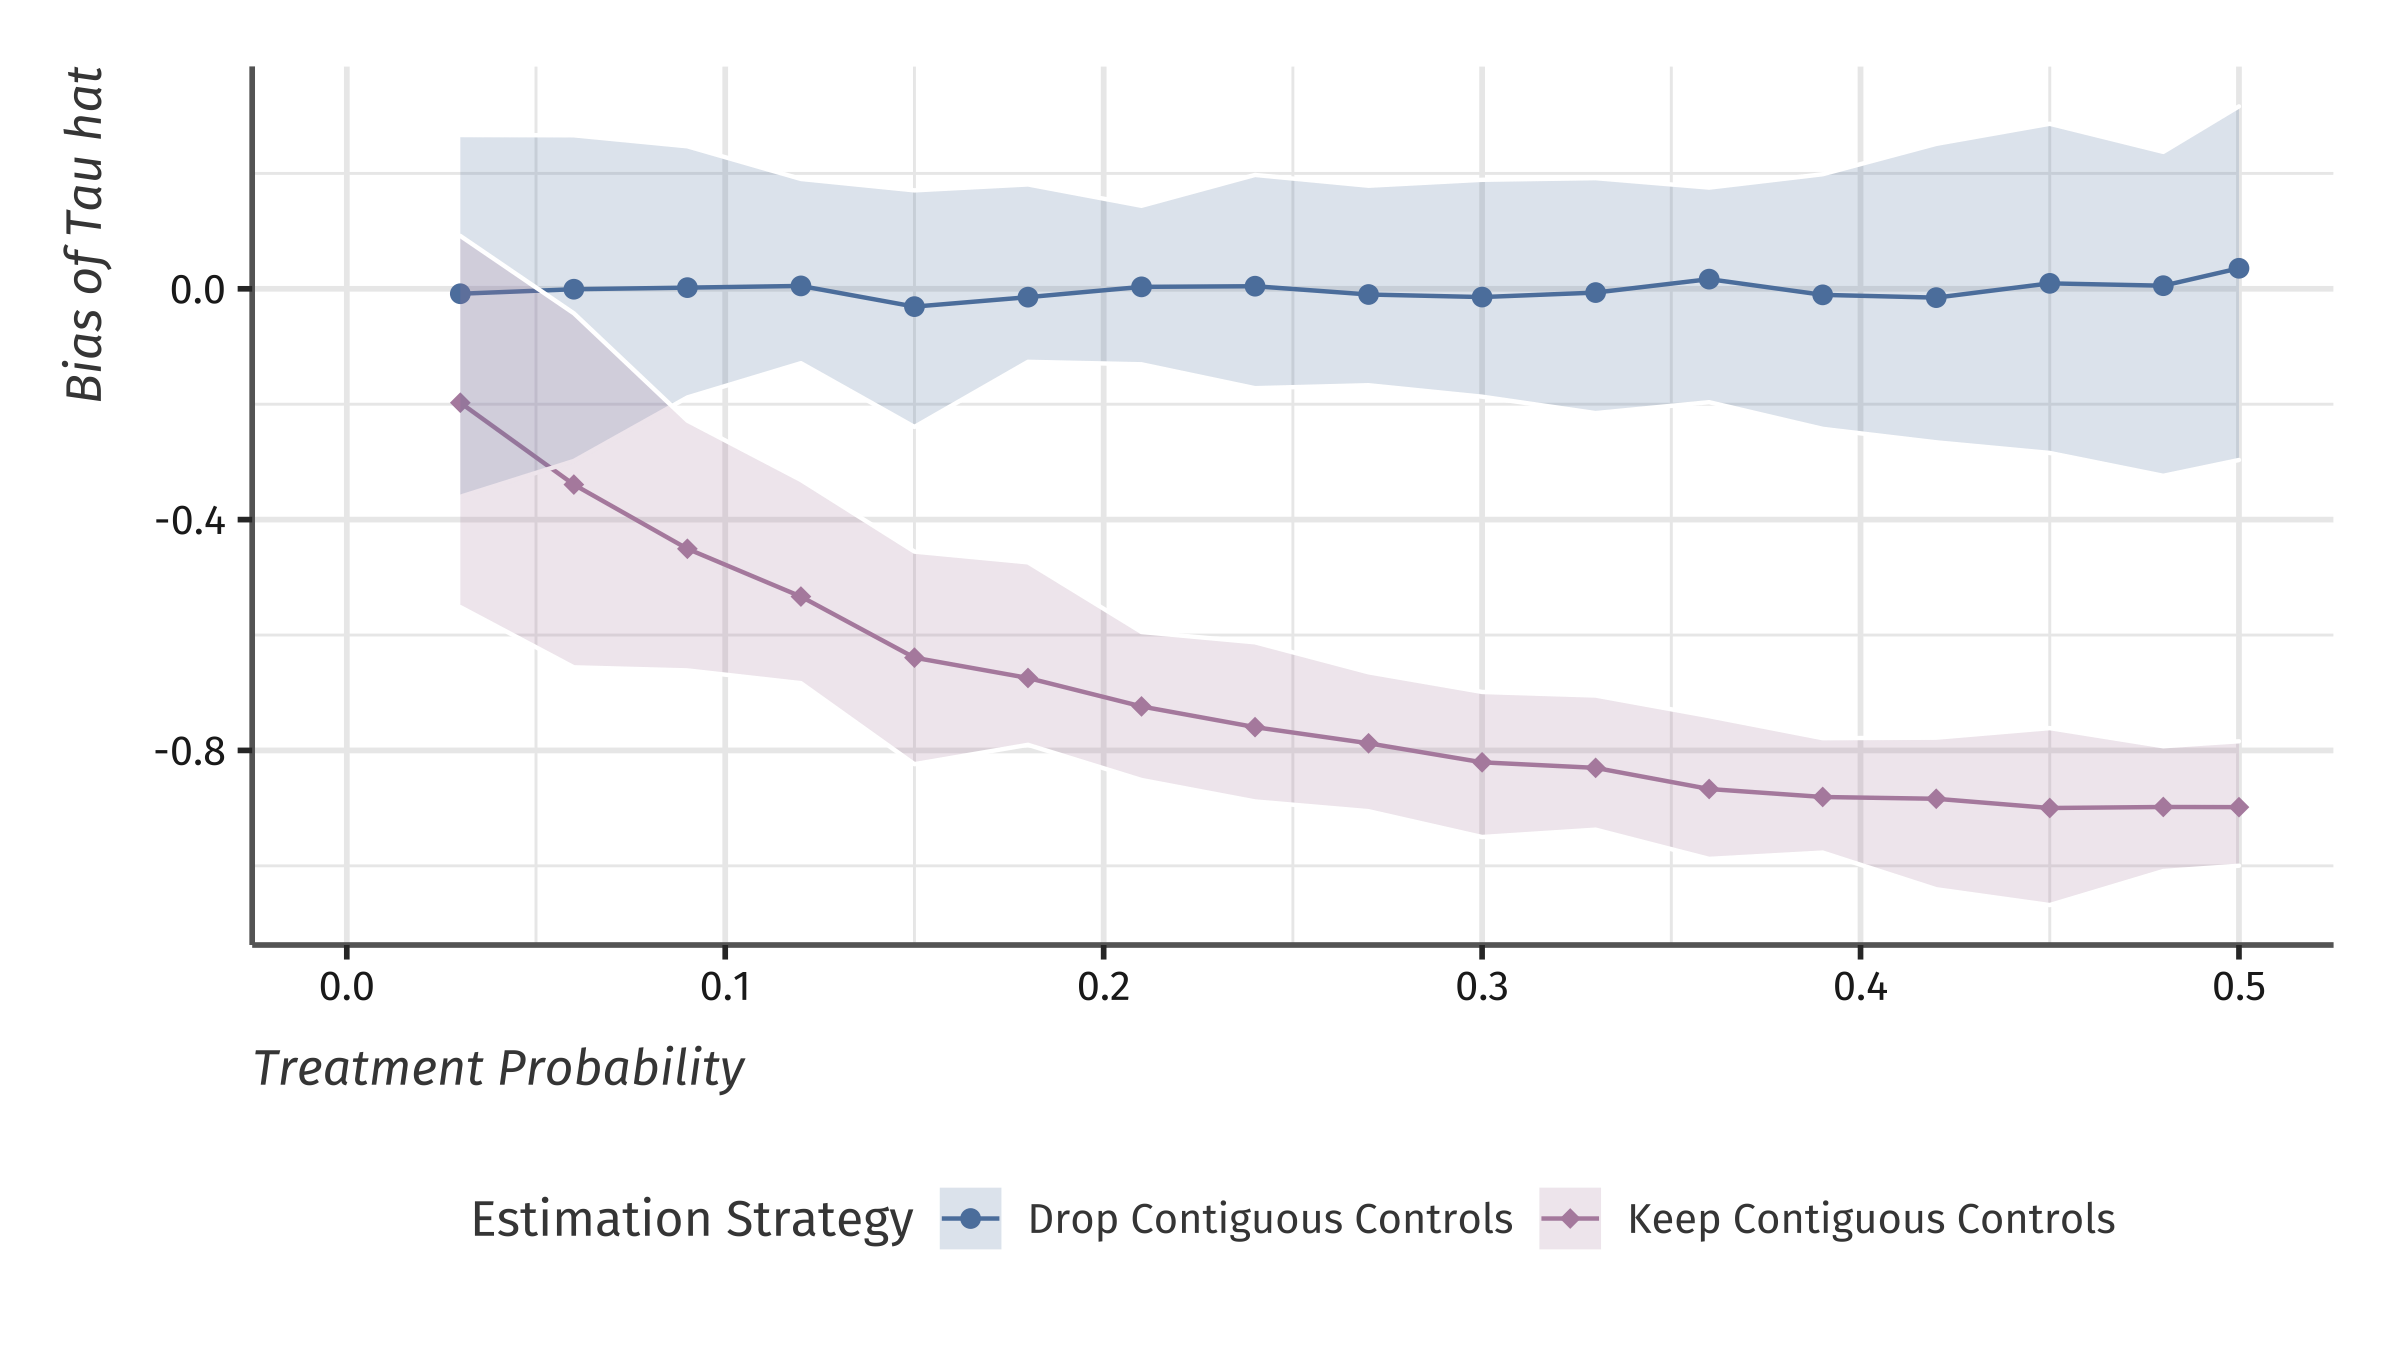
\includegraphics[width=\textwidth]{../../figures/figure-bias_fix.png}
    } 
    {\footnotesize
        \textit{Notes:} This figure plots the bias of $\hat{\tau}$ found from estimating (\ref{eq:twfe}) for data generated as described in the text and Equation \ref{eq:dgp1}. Each point corresponds to the average bias for the given treatment probability and the band is the 95 percent empirical confidence interval over 1000 simulations. The line with diamond markers estimates with all control units. The line with circle markers removes control units that share a border with a treated county. 
    }
\end{figure}

The size of the bias from estimating the two-fixed effects model, (\ref{eq:twfe}), at different treatment probabilities are presented in Figure \ref{fig:bias_as_treat_prob} as the line with diamond markers. Each point represents a set of 10,000 simulation and displays the mean bias as well as a 95 percent empirical confidence interval. As displayed in the figure, even for a low treatment probability of three percent, the bias is quite large with a 95 percent empirical confidence interval between -0.28 and -0.75. As treatment frequency increases, the bias increases as well but at a slower rate due to fewer additional control units receiving spillover units. The slow increase in bias is in part due to the assumption that spillovers are not additive in the number of nearby units treated.

A common solution in the literature is to remove control units from the estimated sample that are most likely to be affected by spillovers. To do this, I remove contiguous control counties which is a close, but misspecificied, measure of $h(\vec{D}, i)$. The results are shown in Figure \ref{fig:bias_as_treat_prob} by the line with circle markers. Even though the exposure mapping is misspecified, contiguous counties approximates the true exposure mapping well enough such that the bias stays centered constantly around zero as most control units experiencing spillovers are removed. However, if the distance cutoff $\bar{d}$ were larger, more control units would remain in the sample that experience non-zero exposures. In this case, the bias would fall between the two lines.

There is a trade-off between the bias and the variance of the estimator when using this methodolgy. As the treatment probability increases, the number of control units removed increases as well. This naturally yields a more variable estimator as seen in the wider 95 percent empirical confidence intervals in Figure \ref{fig:bias_as_treat_prob}. This trade-off can be avoided altogether by parameterizing the spillovers and including them in estimation directly.


% -----------------------------------------------------------------------------
\subsection{Spillovers onto Control and Treated Units}
% ------------------------------------------------------------------------------

For the following simulation, I will add in spillovers onto also treated units with $\beta_{\text{spill, treat}} = -0.5$. The DGP is as follows 
\begin{equation}\label{eq:dgp2} 
    y_{it} = \mu_t + \mu_i + 2 D_{it} + (1-D_{it}) \text{Near}_{it} - 0.5 D_{it} \text{Near}_{it} + \varepsilon_{it}   
\end{equation} 
The proportion of treated units affected by the spillover depends on the spatial autocorrelation of the treatment assignment. In empirical applications, it is often the case that treatment assignment is concentrated in specific areas which yields higher proportion of treated units receiving spillover effects.

\begin{figure}[tbh!]
    \caption{Example of Kriging Field}
    \label{fig:kriging}
    \begin{center}
        \resizebox{0.8\textwidth}{!}{
            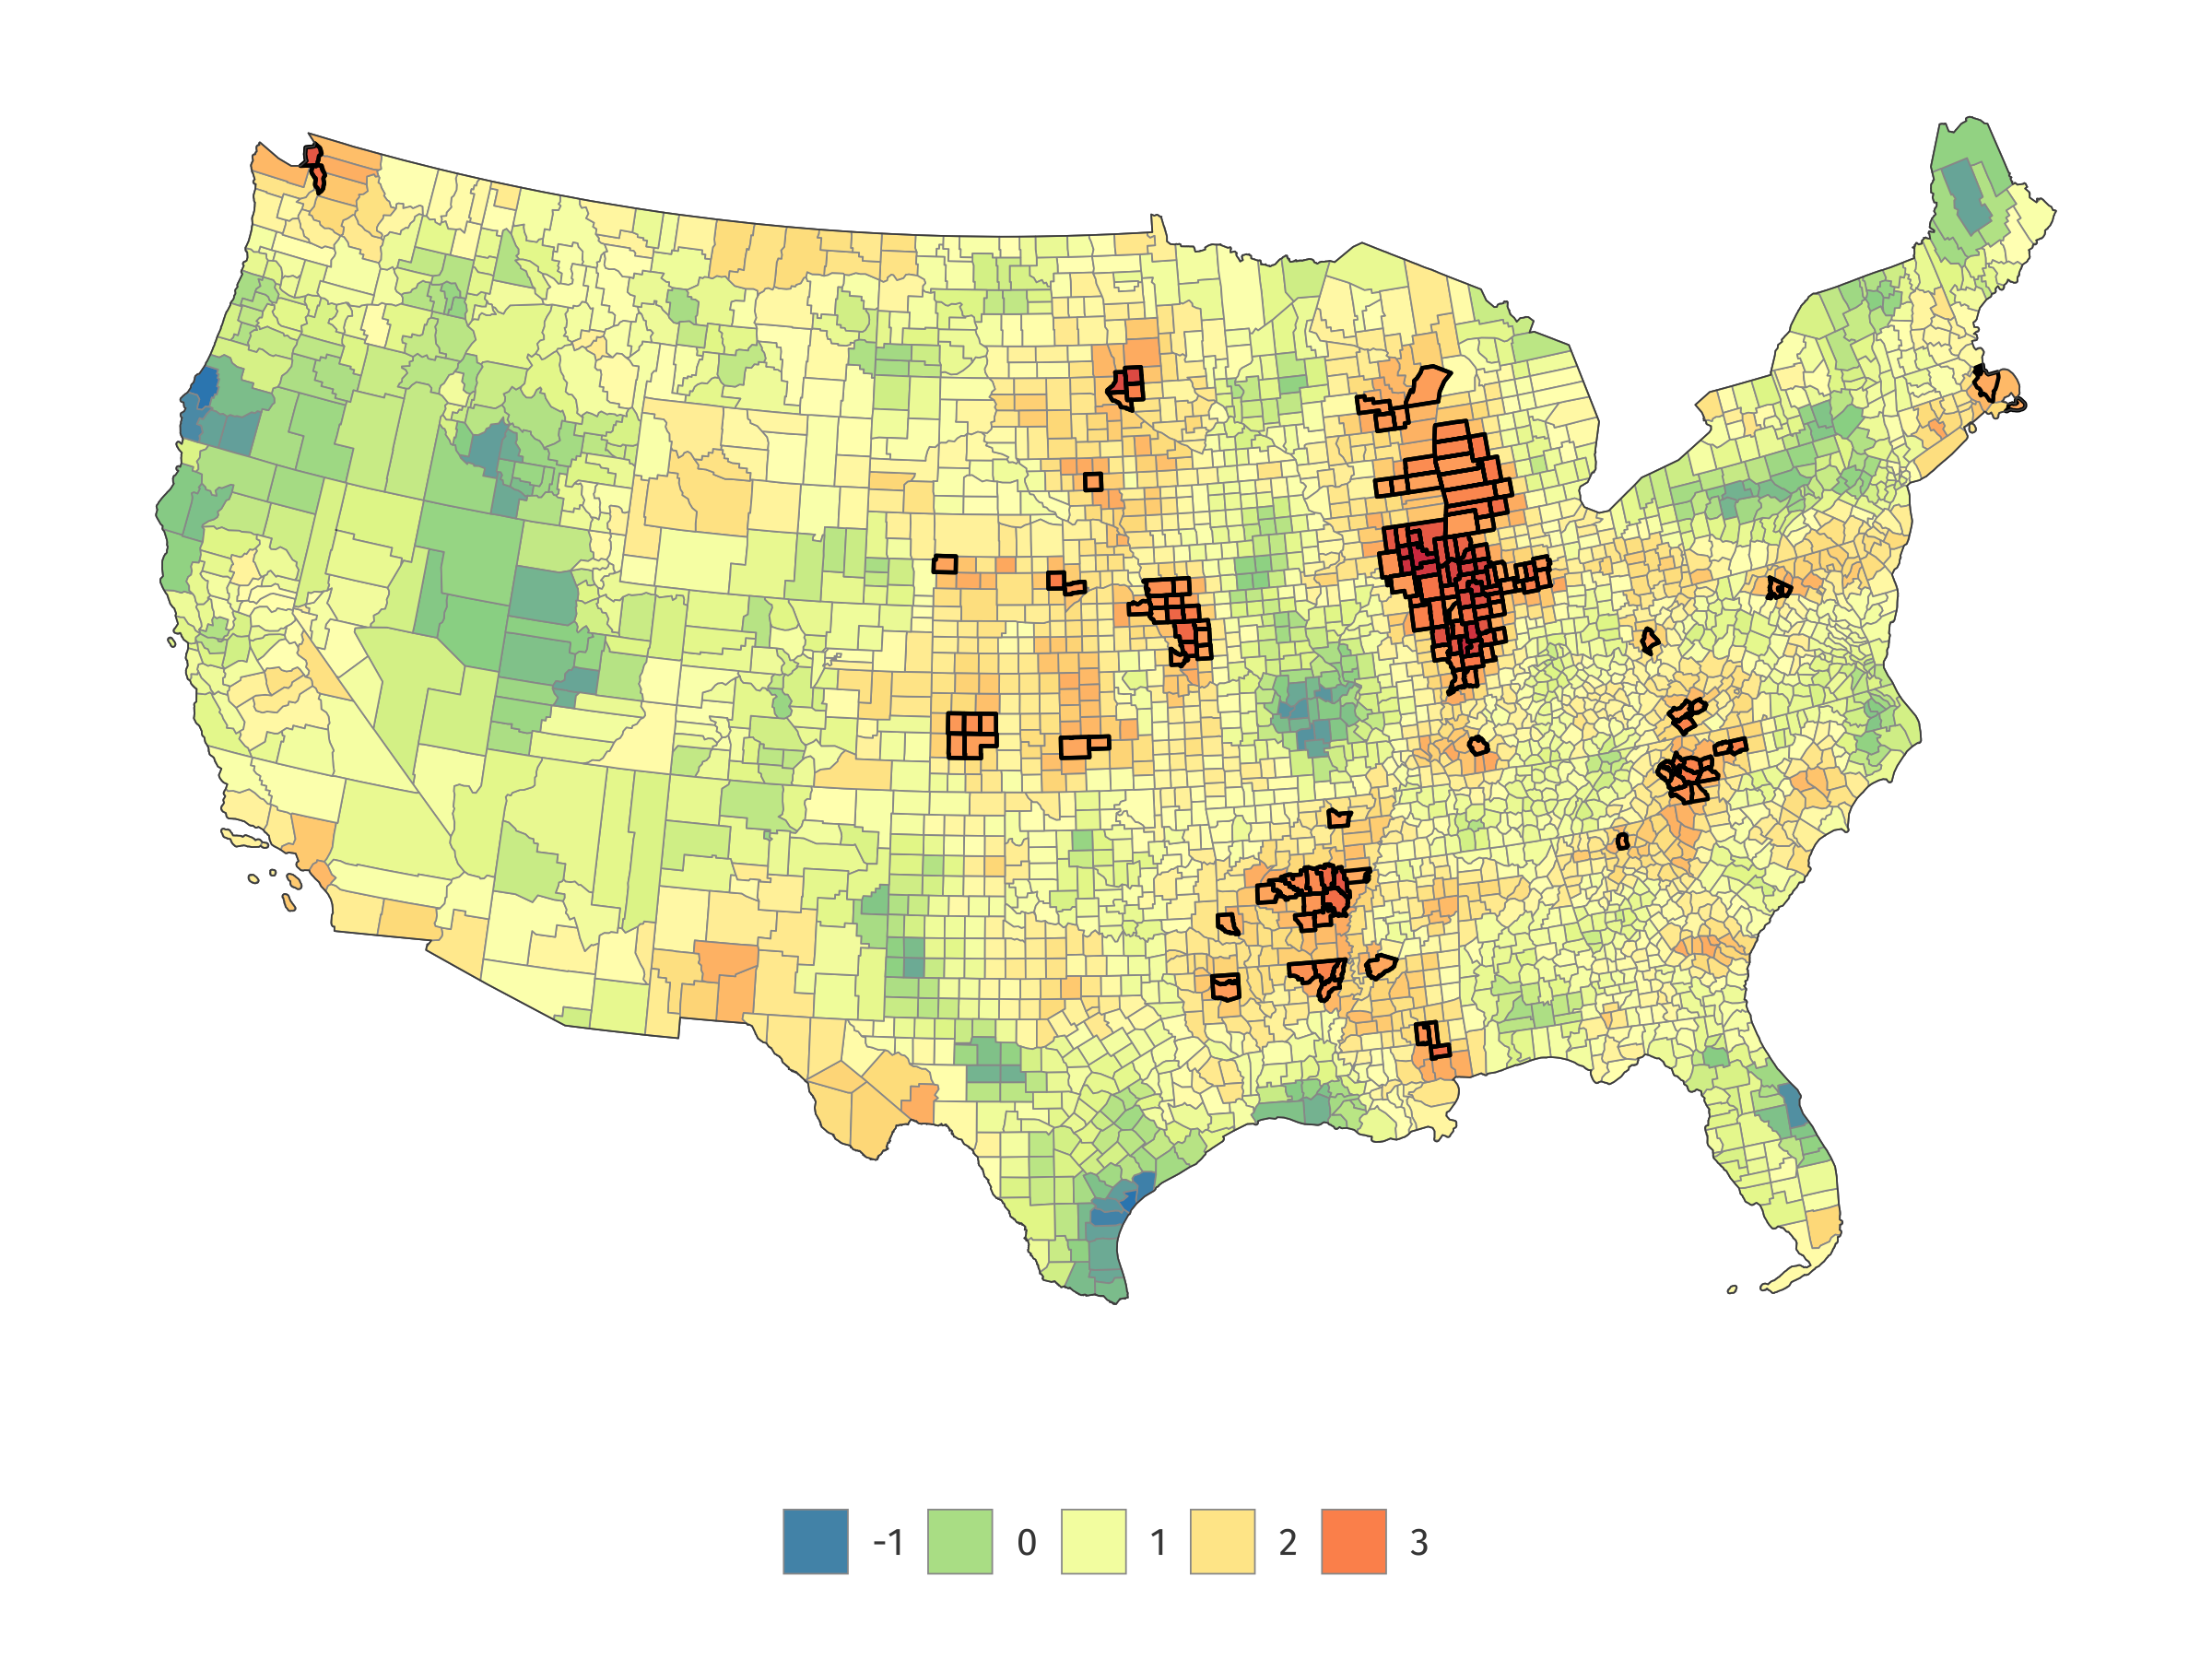
\includegraphics{../../figures/figure-krig.png}
        } 
    \end{center}

    {\footnotesize
        \textit{Notes:} This figure plots an example of a kriging simulation using the `gstat' package in R using an exponential variogram. The outlined counties are in the top ten percent of values for this simulation. 
    }
\end{figure}

\begin{figure}[tbh!]
    \caption{Bias of $\hat{\tau}$ at Different Levels of Spatial Autocorrelation}
    \label{fig:bias_spatial_autocorr}
    {\centering
        \resizebox{\textwidth}{!}{
            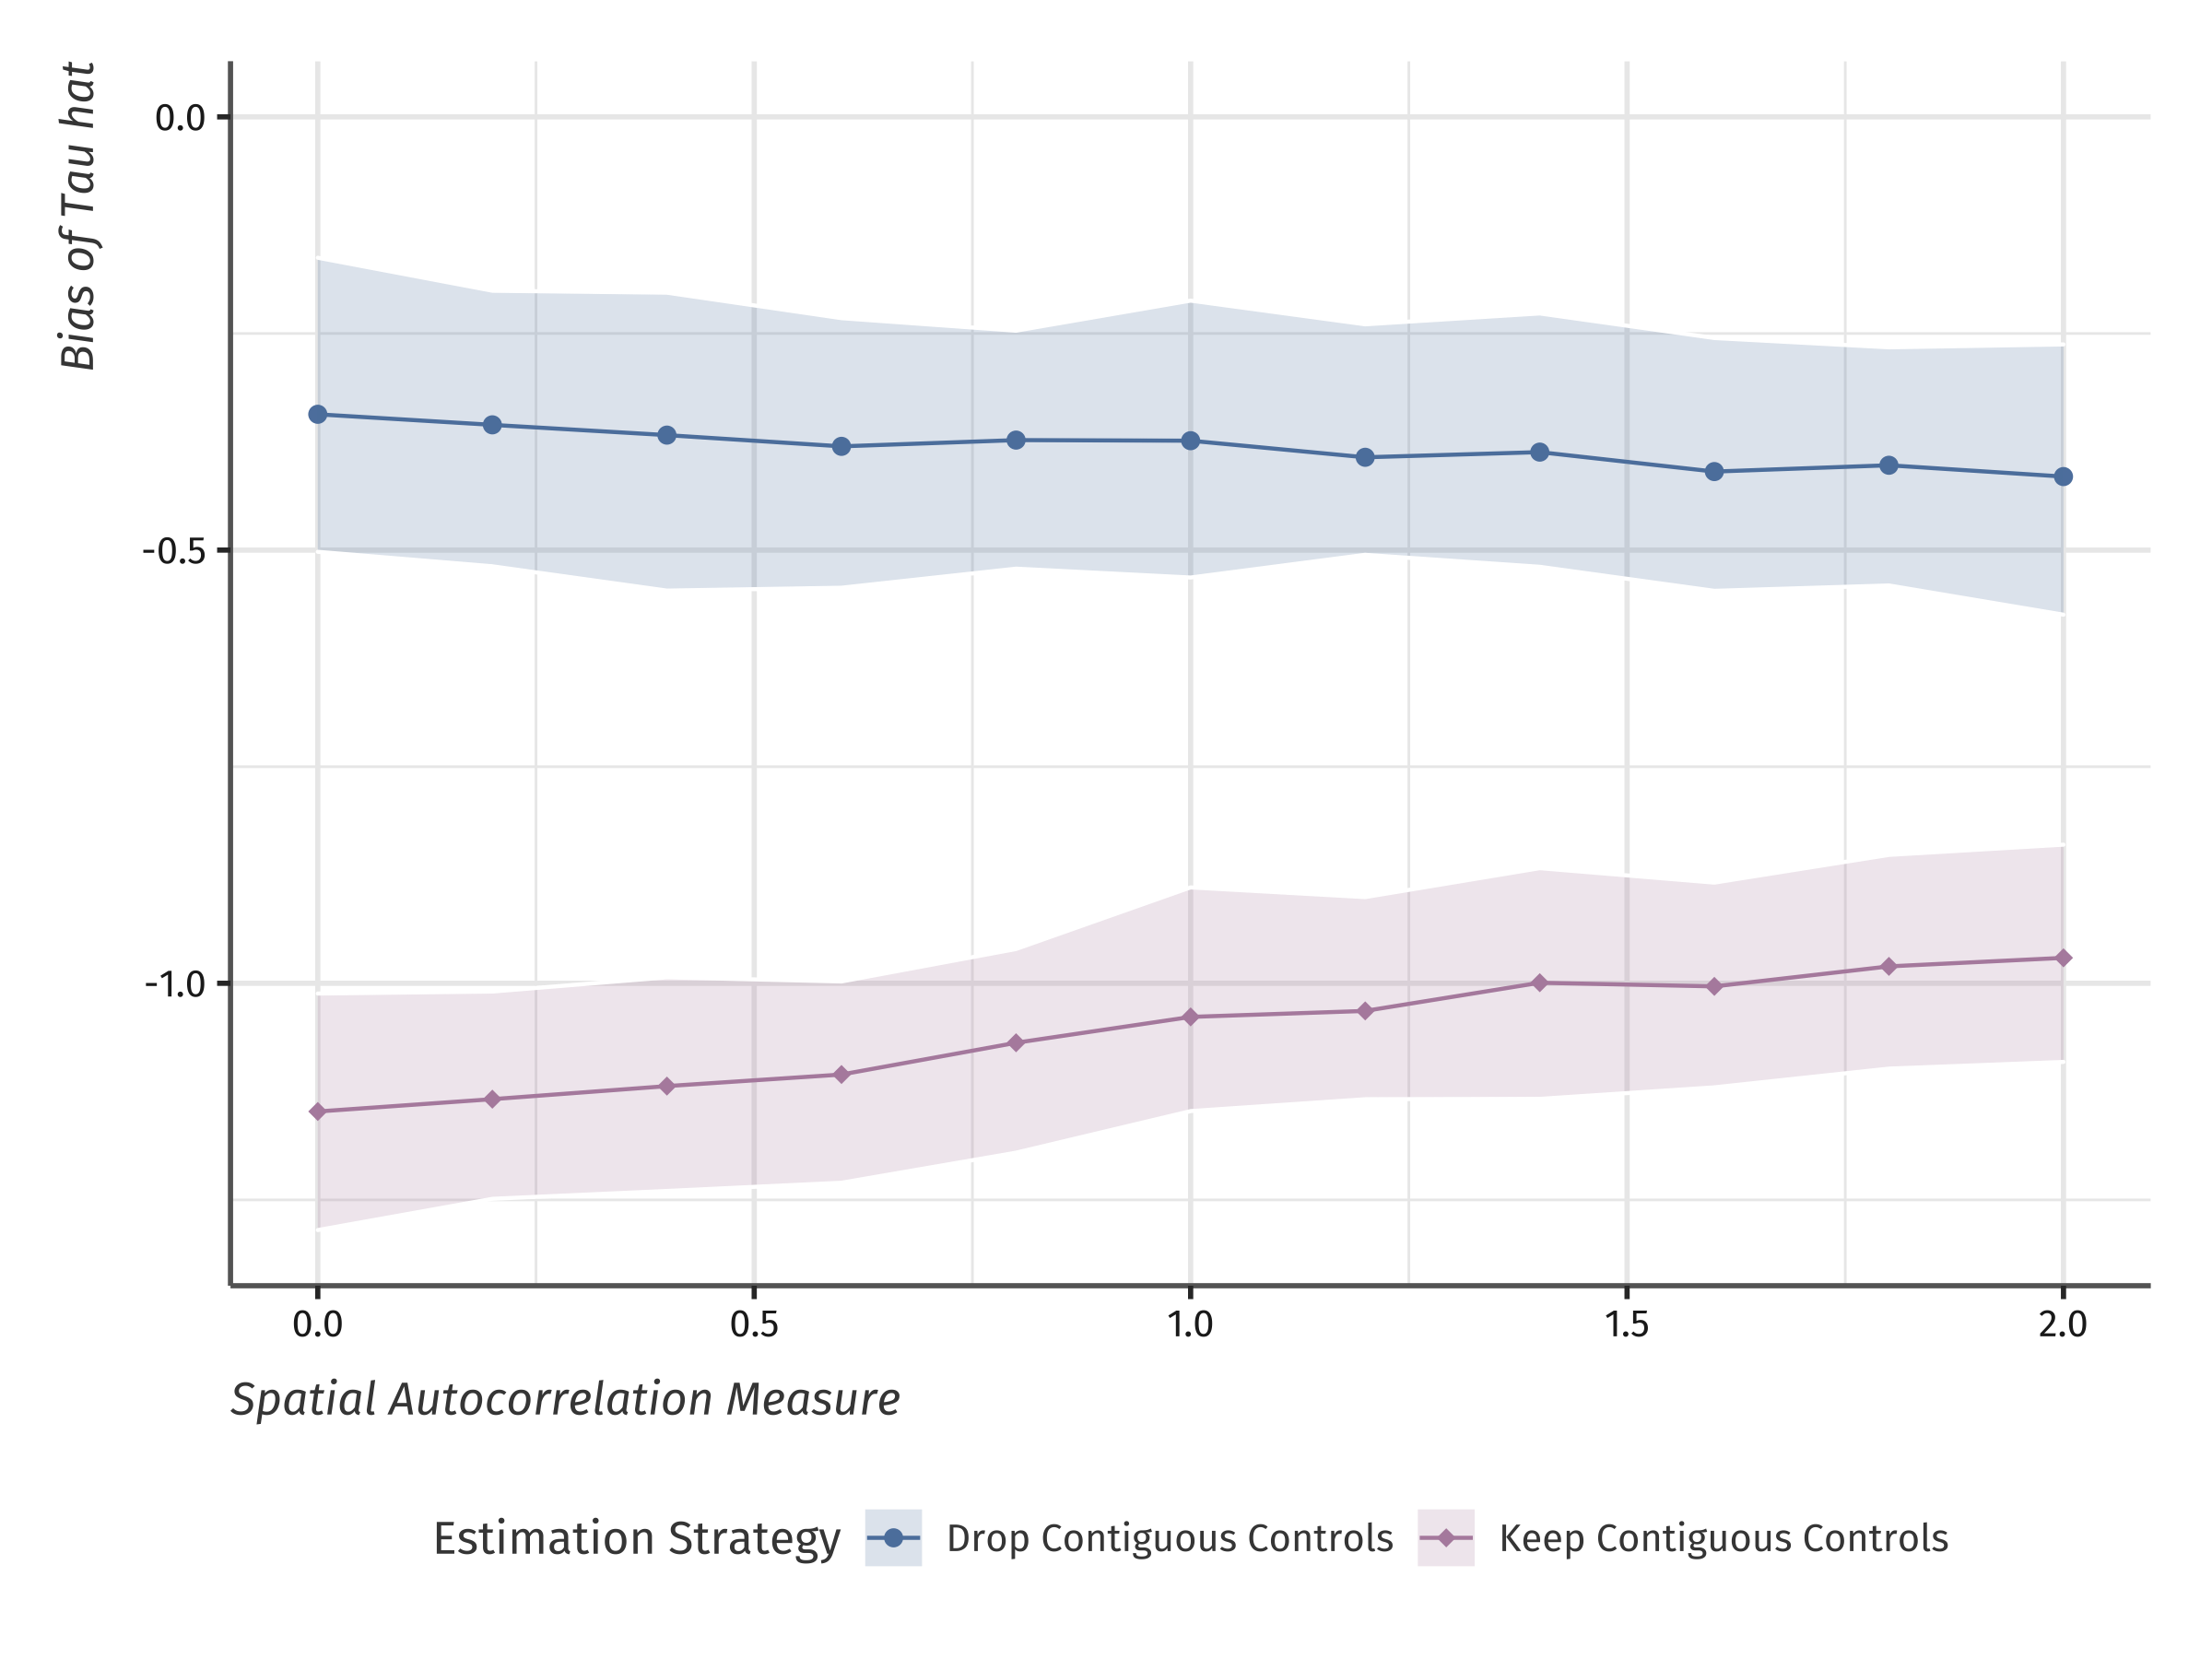
\includegraphics{../../figures/figure-bias_fix_spatial_autocorr.png}
        } 
    }

    {\footnotesize
        \textit{Notes:} This figure plots the bias of $\hat{\tau}$ found from estimating (\ref{eq:twfe}) for data generated as described in the text and Equation \ref{eq:dgp2}. Treatment probability is assigned according to the method described by the text and (\ref{eq:cond_prob}). Each point corresponds to the average bias for the given Zone Plus and the band is the 95 percent empirical confidence interval over 1000 simulations. The line with diamond markers estimates with all control units. The line with circle markers removes control units that share a border with a treated county. 
    }
\end{figure}

In order to model spatial autocorrelation of treatment, I turn to a method from geosciences called `kriging'. Kriging generates a Gaussian field for a large grid of points across the entire United States where the spatial autocorrelation of the points is described by a set of parameters. One such field is depicted in Figure \ref{fig:kriging}. For a given field, I find the counties in the top ten percent of values and give these counties a value of $\text{Zone}_i = 1$. Then I assign treatment with a probability that differs based on $\text{Zone}_i$. To avoid changes in bias due to a difference in the number of treated units, the unconditional probability is equal to 5 percent in all simulations. 

To change the spatial autocorrelation of treatment, I use a variable `Zone Plus' to adjust the relative probability of receiving treatment: 
\begin{equation}
    \label{eq:cond_prob}
    P(D_i \ \vert \ \text{Zone}_i) = (.05 + \text{Zone Plus} * \text{Zone}_i) \times \underbrace{\frac{.05}{.05 * .9 + (.05 + \text{Zone Plus}) * .1}}_{\text{Normalize } P(D_i) = 0.05}
\end{equation}
The second term normalizes probabilities so the unconditional probability stays at five percent. In our simulations, Zone Plus ranges from 0 which is the case where $P(D_i \vert \text{Zone}_i) = P(D_i) = 0.05$ to 2 which has $P(D_i \ \vert \ \text{Zone}_i) = 0.01 + 0.41 * \text{Zone}_i$.

The results for the bias of $\hat{\tau}$ are in Figure \ref{fig:bias_spatial_autocorr}. The line with diamond markers is run on the full sample. As the level of spatial autocorrelation increases, the bias surprisingly decreases. The reason for this is that as treatment becomes more concentrated in the `Zones', the number of control units receiving spillovers decreases while the number of treated units receiving spillovers increases. In this particular DGP, the effect of fewer control units on the bias is larger than the bias from more treated units. 

The line with circle markers in Figure \ref{fig:bias_spatial_autocorr} repeats the exercise of dropping control units that share a border with treated units. In the case where spillovers occur on treated units, all bias is not removed when dropping control units. That is because we only remove $\tau_{\text{spill,control}}$ but $\tau_{\text{spill,treated}}$ remains. To remove the second source of bias, it is necessary to acount directly for spillovers in the estimation strategy. 


% ------------------------------------------------------------------------------
% \subsection{Misspecification of Spillovers}
% ------------------------------------------------------------------------------

% @TODO



% ------------------------------------------------------------------------------
\section{Application in Urban Economics}
\label{sec:tva}
% ------------------------------------------------------------------------------

To illustrate the importance of accounting for spatial spillovers in the estimation of treatment effects, I revisit the analysis of the Tennessee Valley Authority (TVA) in \citet{Kline_Moretti_2014}. The TVA program was a large-scale federal investment started in 1934 that focused on modernizing the Tennessee Valley economy. The program focused on electrification through dams and transportation canals in order to improve the manufacturing economy. By the end of WWII, the TVA became the largest single power supplier in the country.\footnote{More details on the program are found in \citet{Kline_Moretti_2014}.} With over \$20 Billion (in 2000 dollars) spent and hundreds of dollars transferred per person in the Authority, the impacts are very likely to cross far past the authority's borders. 

\citet{Kline_Moretti_2014} focus on a set of outcome variables, but I will focus on three in the analysis. The first two are (the log of) agricultural and manufacturing employment and the last is (the log of) median household income. Since the TVA focused on manufacturing employment, the authors predict that employment will grow in manufacturing and shrink in agricultural. Since manufacturing jobs pay more on average, the median household income will therefore grow. 

In \citet{Kline_Moretti_2014}, they discuss the nature of spillovers that can occur. For agriculture employment, the authors claim that improved wages in the Authority will draw agriculture workers out of nearby counties. Hence they predict a negative spillover. For manufacturing, the sign is ambiguous. There could be positive spillovers if electrification brought cheap power to the neighboring areas. Also, agglomeration effects increase manufacturing employment in nearby counties.\footnote{\citet{Duranton_Puga_2003} give theoretical motivations for different sources of agglomeration. In this context, agglomerations due to `sourcing' is most likely. When the Authority has a large increase in manufacturing, they develop resource supply chains that in turn make inputs cheaper for neighboring counties.} However, manufacturing could decline if firms chose to locate in the Authority that would have, in the absence of the program, decided to locate in nearby counties. 

The analysis in \citet{Kline_Moretti_2014} begins by comparing long-differences in county-level outcomes from 1940 to 2000 between treated counties in the Authority and control counties outside. The primary difference-in-differences specification is
\begin{equation}\label{eq:tva}
    y_{c, t} = \mu_c + \mu_t + \tau \text{TVA}_c \times \text{Post}_t + X_{c, 1940} \times \text{Post}_t \gamma + \epsilon_{c,t},
\end{equation}
where $c$ denotes county, $\text{TVA}_c$ is an indicator variable for being in the Authority, $\text{Post}_t$ equals one when $t = 2010$ and equals zero when $t = 1940$, and $y$ is a set of outcome variables.\footnote{Outcome variables are all in logs and include population, average manufacturing wage, agricultural employment, manufacturing employment, value of farm production, median family income, and median housing value. The text writes the equivalent first-differences regression: \[ 
    y_{c, 2000} - y_{c, 1940} = \alpha + \text{TVA}_c \tau + X_{c, 1940} \gamma + (\varepsilon_{c, 2000} - \varepsilon_{c, 1940}). 
\]} Pre-treatment control variables, $X_{c,1940}$, are interacted with $\text{Post}_t$ to allow for places to be on different long-term trends.\footnote{See footnote 8 in \citet{Kline_Moretti_2014} for a full listing of control variables.} 

\citet{Kline_Moretti_2014} estimate Equation \ref{eq:tva} to identify the `local effect' of the TVA -- what I am calling the `direct effect'. However, their point estimates compare, in part, changes in outcomes in TVA counties with changes in outcomes for neighboring counties that likely were impacted by the large-scale program. Their identification strategy depends \emph{explicitly} on a parallel counterfactual trends assumption after controlling for covariates and \emph{implicitly} on the SUTVA assumption. 

As described above and estimated below, the program likely induced manufacturing and agricultural employment effects in nearby counties. By comparing counties inside the Authroity to counties on the other side of the border, the authors likely underestimate the negative effect on agricultural employment while the bias in the manufacturing effect and median family income is theoretically ambiguous. The authors do recognize the problem of these comparisons and remove counties that share borders with the authority's, but due to the scale of the program, the spillovers are likely to extend further than this and appear to do so in the empirical analysis below.  

The authors use an Oaxaca-Blinder estimator on the first differences and the results of \citet{Kline_2011} show that this estimator is a weighted difference-in-differences. The weights can be seen in Figure III of their text, but generally counties close to the TVA are upweighted. However, in Table \ref{tab:tva} below, I will show their estimator does not differ much from the standard difference-in-differences results since the weights are not that different from uniform weights. 

In order to more likely satisfy the paralell trends assumption, the run a logistic regression to predict being in the TVA based on their set of control variables $X_{c, pre}$ and keep only observations in the top 75\% of predicted probability. The counties used in the sample are presented in Figure \ref{fig:tva_sample}. 

\begin{figure}[tb!]
    \caption{TVA Effective Sample and Spillover Variables}
    \label{fig:tva_sample}

    {\centering
        \resizebox{\textwidth}{!}{
            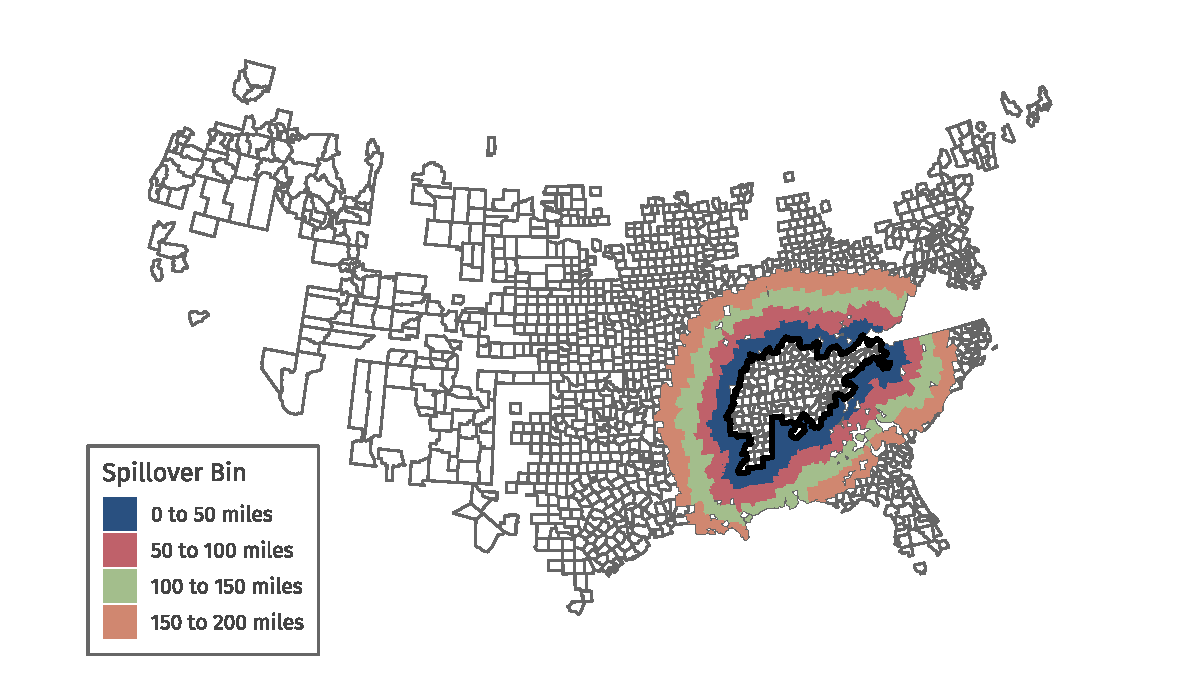
\includegraphics{../../figures/figure-tva-sample.pdf}
        } 
    }

    {\footnotesize \textit{Notes:} The above figure plots all the counties used in the estimation. Counties that fall within the distance intervals $\{(0, 50], (50, 100], (100, 150]\}$ measured in miles are colored by their respective bin.}
\end{figure}

I extend their analysis to include spatial spillovers in the difference-in-differences specification. To parametrize the exposure mapping, I include a set of indicator variables for being in distance bins away from the Authority. I do this for two reasons. Specifically, I use the following intervals $\text{Dist} = \{(0, 50], (50, 100], (100, 150]\}$ measured in miles and define $\text{Between}(d)$ as an indicator for being within the interval $d \in \text{Dist}$ away from the Authority. Figure \ref{fig:tva_sample} displays the three spillover variables by filling in each distance bin in a different color. As discussed above, I suspect the spillover effects to change with distance to the Authority, hence I allow the effect to be seperately identified in bins. I keep the number of bins small to improve precision of spillover estimates. 

The specification with spillovers is given as follows:  
\begin{equation}\label{eq:tva_spillover}
    y_{i, 2000} - y_{i, 1940} = \alpha + \text{TVA}_i \tau + \sum_{d \in \text{Dist}} \text{Between}(d)\delta_d + X_{i, 1940} \beta + (\varepsilon_{i, 2000} - \varepsilon_{i, 1940})
\end{equation} 
The coefficients $\delta_d$ measure the spillover effect onto control units at different distances from the Authority. If specification \ref{eq:tva_spillover} is correctly specified, then $\hat{\tau}$ will be an unbiased estimate for what the authors call the `local' effect. As shown above, minor misspecification will remove some but not all of the bias from standard difference-in-differences estimates. 

The results of the analysis are presented in Table \ref{tab:tva}. The first column lists which dependent variable (measured in logs) was used in the row. The following columns contain point estimates for $\tau$ and $\delta_s$ in different specifications and can be interpreted as decadel growth rates in outcomes. The column labeled `Kline \& Moretti (2011)' use an Oaxaca-Blinder estimator while the column labeled difference-in-differences uses an ordinary least squares estimator for Equation \ref{eq:tva}. The two columns are very close in magnitude to each other. They find a decline in agricultural employment of about $5.6\%$ per decade, an increase in manufacturing employment of about $6.1\%$ per decade, and an increase in median family income of about $2.2\%$ per decade. 


% \begin{landscape}
% \thispagestyle{lscaped}
\begin{table}[!tb]
    \caption{Effects of Tennessee Valley Authority on Decadel Growth}
    \label{tab:tva}
    \renewcommand{\arraystretch}{1}

    \begin{adjustbox}{width = 1.15\textwidth, center}
        \begin{threeparttable}
            \begin{tabular}{@{} lc@{\extracolsep{20pt}}cc@{\extracolsep{4pt}}ccc @{}}
                % Head
                \toprule

                & \multicolumn{1}{c}{\textbf{Kline \& Moretti (2011)}} &
                \multicolumn{1}{c}{\textbf{Diff-in-Diff}} & \multicolumn{4}{c}{\textbf{Diff-in-Diff with Spillovers}} \\ 
                \cmidrule{2-2} \cmidrule{3-3} \cmidrule{4-7} 
                & & & & TVA between & TVA between & TVA between \\ 
                & TVA & TVA & TVA & 0-50 mi. & 50-100 mi. & 100-150 mi. \\ 
                \textit{Dependent Var.} & (1) & (2) & (3) & (4) & (5) & (6) \\
                
 
                % Body
                \midrule
                
                
                 Population                  &    $0.0052$    &    $0.0053$    &    $-0.0040$   &    $-0.0212$   &    $-0.0077$   &    $-0.0053$   \\
                             &   $(0.0099)$   &   $(0.0090)$   &   $(0.0089)$   &   $(0.0179)$   &   $(0.0125)$   &   $(0.0123)$   \\
 Average manufacturing wage  &    $0.0064$    &  $0.0070^{**}$ &  $0.0075^{*}$  &    $0.0022$    &    $-0.0037$   &    $0.0023$    \\
                             &   $(0.0048)$   &   $(0.0030)$   &   $(0.0045)$   &   $(0.0047)$   &   $(0.0040)$   &   $(0.0047)$   \\
 Agricultural employment     & $-0.0561^{***}$& $-0.0514^{***}$& $-0.0678^{***}$& $-0.0310^{**}$ &    $-0.0112$   & $-0.0252^{***}$\\
                             &   $(0.0100)$   &   $(0.0087)$   &   $(0.0102)$   &   $(0.0123)$   &   $(0.0094)$   &   $(0.0084)$   \\
 Manufacturing employment    & $0.0606^{***}$ & $0.0560^{***}$ &  $0.0461^{**}$ &    $-0.0104$   &    $-0.0128$   &  $-0.0248^{*}$ \\
                             &   $(0.0170)$   &   $(0.0187)$   &   $(0.0210)$   &   $(0.0205)$   &   $(0.0257)$   &   $(0.0147)$   \\
 Value of farm production    &    $0.0024$    &    $-0.0060$   &    $-0.0184$   &    $-0.0188$   &    $-0.0101$   &    $-0.0266$   \\
                             &   $(0.0245)$   &   $(0.0269)$   &   $(0.0313)$   &   $(0.0252)$   &   $(0.0227)$   &   $(0.0176)$   \\
 Median family income        & $0.0219^{***}$ & $0.0191^{***}$ &  $0.0196^{**}$ &    $0.0056$    &    $-0.0062$   &    $-0.0011$   \\
                             &   $(0.0061)$   &   $(0.0067)$   &   $(0.0077)$   &   $(0.0079)$   &   $(0.0060)$   &   $(0.0032)$   \\
 Median housing value        &    $-0.0020$   &    $-0.0055$   &    $-0.0029$   &    $0.0039$    &    $0.0068$    &    $0.0006$    \\
                             &   $(0.0107)$   &   $(0.0091)$   &   $(0.0091)$   &   $(0.0163)$   &   $(0.0132)$   &   $(0.0063)$   \\

                
                \bottomrule
            \end{tabular}
            
            % Notes 
            \begin{tablenotes}\footnotesize
                \item \textit{Notes.} Each row corresponds to an outcome variable. Each cell is the point estimate and the standard error for the variable described in the column title. All standard errors are clustered at the state-level. The column labeled \citet{Kline_Moretti_2014} replicates the Oaxaca-Blinder estimator found in column (3) of Table III. The column labeled `Diff-in-Diff' estimates Equation \ref{eq:tva} by OLS. The final four columns labeled `Diff-in-Diff with Spillovers' are estimates from Equation \ref{eq:tva_spillover}.
                
                \item $^{*} p< 0.1$; $^{**} p < 0.05$; $^{***} p < 0.01$.
            \end{tablenotes}
        \end{threeparttable}
    \end{adjustbox}
\end{table}
%\end{landscape}

Turning to the last four columns that estimate Equation \ref{eq:tva_spillover}, column (3) contains a point estimate for $\tau$ and and columns (4)-(6) contain point estimates of the spillover effects $\delta_d$. For agricultural employment, our point estimates show there was a decline in agriculture employment in control units near the Authority. For control units between 0 and 50 miles, column (4) indicates a decline in agricultural employment of $3.1\%$. Between 50 and 100 miles the point estimate is $-1.1\%$ and between 100 and 150 miles, the point estimate is $-2.5\%$. This is likely due to the fact that higher paying manufacturing jobs within the Authority drew migrants from nearby counties. Because the spillovers onto the control counties is negative, the original difference-in-differences estimator was positively biased. The new point estimate indicates a decline of agricultural employment of about $6.8\%$ per decade compared to $5.1\%$ in the standard difference-in-difference specification. 

For manufacturing, our point estimates for spillovers in column (4)-(6) are not statistically significant, but the signs on all three spillover estimates suggest that neighboring counties had a potentially negative spillover effect. Since there is little to no spillovers present, the new point estimate in column (3) of $4.6\%$ is not too far from the standard difference-in-differences estimate of $5.6\%$. Similarly, there is not a significant spillover on median family income. The point estimate therefore stays the same between the standard and spillover-adjusted difference-in-differences estimate of about $1.9\%$. 

These results show that including spillovers in the estimation of direct treatment effects is potentially important and in the case of agricultural employment can lead to \emph{significant} differences in treatment effect estimates. Analysis of place-based policies that do not account for the fact that treatment effects can spillover beyond the borders of treated areas can potentially be biased. The above results suggest this can over or underestimate the size of the effects depending on the sign of the spillovers. 






% ------------------------------------------------------------------------------
\newpage \printbibliography%
% ------------------------------------------------------------------------------


% ------------------------------------------------------------------------------
\newpage \appendix 
\renewcommand{\thetable}{\Alph{section}.\arabic{table}}
\renewcommand{\thefigure}{\Alph{section}.\arabic{figure}}
% ------------------------------------------------------------------------------

% ------------------------------------------------------------------------------
\section{Proofs}
\label{sec:proofs}
% ------------------------------------------------------------------------------

\textbf{Proof of Theorem \ref{thm:bias}}
\begin{align*}
    \mathbb{E}\left[ \hat{\tau} \right] &= \underbrace{\mathbb{E}\left[ Y_{i1} - Y_{i0} \mid D_i = 1 \right] - \mathbb{E}\left[ Y_{i1} - Y_{i0} \mid D_i = 0 \right]}_{\text{Difference-in-Differences}} \\
    &= 
    \mathbb{E}\left[ Y_{i1}(1, h(\vec{D}, i)) - Y_{i0}(0, \vec{0})  \mid D_i = 1 \right] - \mathbb{E}\left[ Y_{i1}(0, h(\vec{D}, i)) - Y_{i0}(0, \vec{0}) \mid D_i = 0 \right] \\
    &= 
    \mathbb{E}\left[ Y_{i1}(1, h(\vec{D}, i)) - Y_{i0}(0, \vec{0})  \mid D_i = 1 \right] - \mathbb{E}\left[ Y_{i1}(0, h(\vec{D}, i)) + Y_{i1}(0, \vec{0}) - Y_{i1}(0, \vec{0}) - Y_{i0}(0, \vec{0}) \mid D_i = 0 \right] \\
    &= 
    \mathbb{E}\left[ Y_{i1}(1, h(\vec{D}, i)) - Y_{i0}(0, \vec{0})  \mid D_i = 1 \right] - \mathbb{E} \left[ Y_{i1}(0, \vec{0}) - Y_{i0}(0, \vec{0}) \mid D_i = 0 \right] \\ 
    &\quad - \mathbb{E} \left[ Y_{i1}(0, h(\vec{D}, i)) - Y_{i1}(0, \vec{0})\mid D_i = 0 \right] \\ 
    &= 
    \mathbb{E}\left[ Y_{i1}(1, h(\vec{D}, i)) - Y_{i0}(0, \vec{0})  \mid D_i = 1 \right] - \mathbb{E} \left[ Y_{i1}(0, \vec{0}) - Y_{i0}(0, \vec{0}) \mid D_i = 1 \right] \\
    &\quad - \mathbb{E} \left[ Y_{i1}(0, h(\vec{D}, i)) - Y_{i1}(0, \vec{0})\mid D_i = 0 \right] \\  
    &= \mathbb{E}\left[ Y_{i1}(1, h(\vec{D}, i)) - Y_{i0}(0, \vec{0}) - Y_{i1}(0, \vec{0}) + Y_{i0}(0, \vec{0})\mid D_i = 1 \right] - \mathbb{E} \left[ Y_{i1}(0, h(\vec{D}, i)) - Y_{i1}(0, \vec{0})\mid D_i = 0 \right]\\
    &= \mathbb{E}\left[ Y_{i1}(1, h(\vec{D}, i)) - Y_{i1}(0, \vec{0}) \mid D_i = 1 \right] - \mathbb{E} \left[ Y_{i1}(0, h(\vec{D}, i)) - Y_{i1}(0, \vec{0})\mid D_i = 0 \right]\\
    &= \mathbb{E}\left[ Y_{i1}(1, h(\vec{D}, i)) + Y_{i1}(1, \vec{0}) - Y_{i1}(1, \vec{0}) - Y_{i1}(0, \vec{0})\mid D_i = 1 \right] - \mathbb{E} \left[ Y_{i1}(0, h(\vec{D}, i)) - Y_{i1}(0, \vec{0})\mid D_i = 0 \right]\\
    &= 
    \mathbb{E} \left[ Y_{i1}(1, \vec{0}) - Y_{i1}(0, \vec{0}) \mid D_i = 1 \right] + \mathbb{E} \left[ Y_{i1}(1, h(\vec{D}, i)) - Y_{i1}(1, \vec{0}) \mid D_i = 1 \right] \\
    &\quad - \mathbb{E} \left[ Y_{i1}(0, h(\vec{D}, i)) - Y_{i1}(0, \vec{0}) \mid D_i = 0 \right] \\
    &= \tau_{\text{direct}} + \tau_{\text{spill,treated}} - \tau_{\text{spill,control}}
\end{align*}








\end{document}